\section{Implementation}

To realize our PGLAS, we have implemented a parallel distributed key/value store, 
PDHT. A novel aspect of this system is its implementation directly on top of the
Portals network interface. The Portals framework provides several low-level 
data abstractions that map nicely onto the PGLAS operations supported by PDHT.

PDHT adopts a one-sided communication model which operates 
with PGAS-like semantics. However, by implementing directly using Portals, we
can take advantage of message-passing features that permit an efficient, 
hardware-offload friendly version of a PGLAS. Some background in the Portals
networking model is helpful in understanding our approach in implementing PDHT.

\subsection{Portals Networking Interface}

% provides several low-level adts for pdht
% one-sided, try to avoid involving processor on the target node
% matching is for MPI, novel application to matching interface
% abstractions for implementing PDHT
% using portals allows us to be hardware offload friendly as compared to 
% traditional PGAS techniques.

The Portals interface provides low-level data abstractions that can be used to
implement both PGAS and message-passing run-times. PDHT relies on a one-sided
communication model that aims to avoid processor involvement on the target
node. Portals supports messaging a {\em matching interface} model intended to
support MPI, two-sided matched send/receive pairs. It also provides a
lightweight {\em non-matching} interface that is intended to support one-sided
communications without the need for the matching and ordering semantics
required by MPI. Our implementation uses a novel application of the Portals
matching interface to provide a one-sided model that is the basis of the PDHT
PGLAS. It is useful to describe several Portals concepts and abstractions to
understand the implementation approach used by PDHT.

% use figure* to span both cols
\begin{figure}[ht]
  \centering
  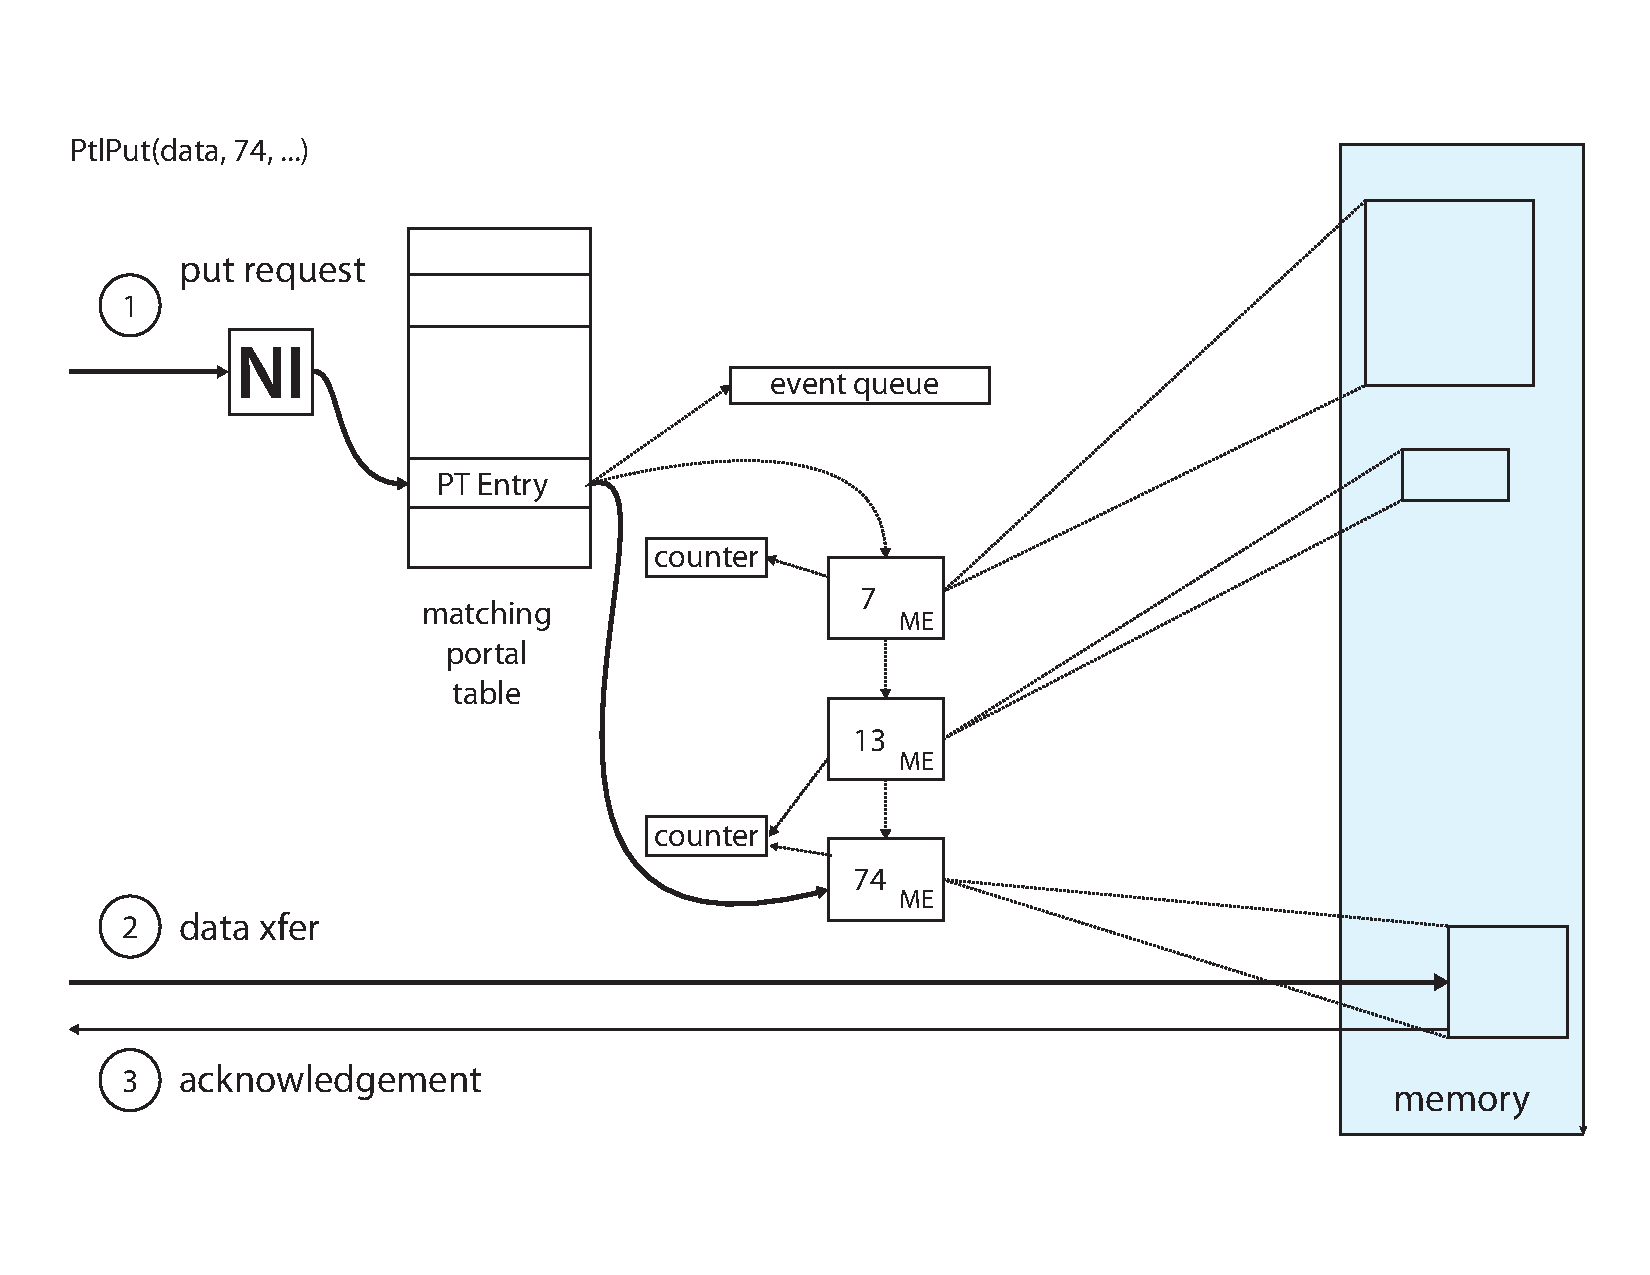
\includegraphics[width=3in]{figs/portals_put}
  \caption{Portals data abstractions used in for a matching interface {\tt put} operation}
  \label{fig:portals_put}
\end{figure}

Portals defines two distinct roles for communication operations. The {\em
  initiator} role is assumed by the process that issues a Portals put, get, or
atomic operation. The {\em target} role is assumed by the process that receives
these operation requests and is responsible for performing the operation or
sending the requested data.

The Portals {\em network interface} (NI) data structure is a per-process
abstraction of a physical network interface and is configured as a
matching or non-matching interface. The NI is associated with both
initiator and target roles. Initiator processes define a {\em memory
  descriptor} (MD) -- a region of memory used for the put/get/atomic
operations as well as ancillary structures used to track communication
events (such as completion) for these operations.

Target processing is expressed in terms of a {\em portal table}. There is one
portal table for each NI, containing multiple entries that separate and
classify communication channels between endpoints.  Each {\em portal table
  entry} (PTE) is identified by a unique index into the Portal table. The index
for a specific PTE is required for all Portals communication operations. Each
PTE maintains a list of memory regions that are valid for communication
operations as well as an event queue which is used to track target-side
asynchronous notifications.  Some completion information and notifications may
only be visible to the initiator and not the target, or vice versa.

A PTE using the matching interface maintains a list of match-list entries (ME).
Each ME specifies a set of matching criteria and a memory region associated
with the entry. If the match criteria are satisfied, the communication
operation commences working on corresponding memory region. Matching criteria
consist of multiple parameters, including a 64-bit {\em match bits} field
that must be an exact match in order for an incoming request to to proceed
with the given ME. For example, a process may post an {\tt MPI\_Recv()} which
creates a new ME on the target PTE with a specific match bits value. Later,
another process would issue an {\tt MPI\_Send()} communication request with
the same match bits that corresponds to the previous receive.

Portals also specifies {\em event queues} and {\em event counters}
used to track data movement in and out of memory regions used by Portals
operations. Events and counters can also log failure events and
other information. Counting events are lightweight operations and only
record the success or failure of a given operation. Full events incur
more overhead but contain detailed information about the event and
the corresponding communication operation.

Event queues may be associated with an MD (initiator-side) or a PTE
(target-side). Event counters are also able to track both initiator
and target events. In contrast to target-side event queues, an event
counter may be associated with a single entry in the match list (an ME), 
rather that for an entire PTE. PDHT typically uses lightweight counting
events to track successful completions and full events to track specific
failures. Detailed descriptions of how event queues and counters are used
within PDHT is discussed below.

Figure~\ref{fig:portals_put} shows a visual representation of the target-side
structures used in an example {\tt PtlPut()} operation using the matching
interface. We assume that the initiator has issued a {\tt PtlPut()} operation
with some data, a PTE index and the match bits set to 74. Upon receiving the
request, the target process searches the match list for the given PTE until a
74 is found or the end of the list is reached. Once a match has been found the
payload data of the {\tt PtlPut} is copied into the memory region associated
with the ME. The completion of this operation may cause an event to be appended
to the PTE event queue or the ME success counter to be incremented. 
Lastly, an acknowledgement message is sent back to the initiator, possibly
generating another full or counting event associated with the MD that
was used to initiate the {\tt PtlPut} operation.

Portals supports two lists for messages, the unexpected list and priority list. 
These are used for the unexpected message queue and posted recieve queue in MPI. Portals supports the 
searching of the local unexpected list through PtlMESearch because of the need to match a MPI\_Recv
call with a message on the local unexpected message queue. However, Portals does not support the searching of 
the local priority list through PtlMESearch. We added functionality to PtlMESearch so it looks for matches
on the local priority list instead of the unexpected list, if specified. This allowed us to find hash table entries without 
calling PtlGet when hash table entries were stored locally. This lead to a 10x speed up in local hash table 
lookups.


\subsection{PDHT Implementation}

% serial vs. parallel approaches
Hash tables can be implemented with a myriad of different techniques, but are
traditionally implemented sequentially as an array of pointers to objects.
Parallel implementations typically distribute table data across nodes,
requiring that the hash table store the entire object and not simply a
reference. 

% parallel programming model
%  - key/value pairs
%  - object can be located anywhere distributed memory, governed
%     solely by hash function
%  - hash function maps key -> rank/offset tuple
%  - two primary operations put/get
%     - if put yields a collision, then object is placed in next
%        available bucket
%     - get returns object, probing as necessary


Our implementation of the PGLAS data model, PDHT, provides a distributed
key/value that is accessed using asynchronous one-sided {\em insert, read,
write,} and {\em atomic update} operations. PDHT uses a traditional hash
function\cite{cityhash} to map an arbitrary user-supplied key to a process rank
and 64-bit hash value. Each key is mapped to a deterministic physical
location within the distributed key/value store.

A PDHT storage structure is represented as a distributed array of objects, with
partitions on all processes. Upon the creation of a new PHDT store, two portal
table entries (PTEs) are allocated. The first PTE contains the {\em pending}
match list, used for insert operations, and the second PTE contains the {\em
active} match list, used for all other operations. The pending match list is
populated with a number of entries that match any incoming communication
requests (i.e. wildcard entries). Each match list entry (ME) in the pending
list is mapped to a distinct memory region located in the local portion of the
distributed array. Pending MEs are marked as use-once and are automatically
unlinked after being written to. In contrast, MEs on the active list may either
be marked as use-once or persistent, depending on the needs of the application.

Every element in the key/value store has a corresponding match list entry. The
ME has a reference to the location in the distributed object array and uses
the 64-bit hash value produced by the hash function as the matching value,
({\em match bits}), in the match list. By using the hashed value of the key
for the match bits field in the ME, the lookup and communication corresponding 
to read operation can be performed entirely by the Portals implementation.

% adding new entries

% data access

% optimizations
%   - 
%  - fence
%  - other features
%    - atomic counter
%    - barrier/reduce/all-reduce/broadcast
%
%- challenges
%  - poll elimination with triggered updates
%  - matchlist length
%    - multiple portal table entries
%    - Portals 4 unordered matching

% HERE
 
%  - migration from pending to active

\subsection{Inserting Objects}

To insert a new element into the hash table, the process first hashes the key,
giving both the target processor rank and the 64-bit match bits field used for
the value. Local insertions are handled as a special-case, by copying the entry
into an available region in the table on the local process and appending a
match list entry onto the active PTE with the match bits set to the value
returned by the hash function.

If the key hashes to a remote process, the process performs a one-sided Portals
put operation on the pending PTE, consuming one of the wildcard entries on the
match list. This process is demonstrated in Figure \ref{fig:put}. The initial
state is shown in Fig. \ref{fig:put}a, with wildcard entries on the pending
match list and available key/value pairs on the active match list. After the
put operation completes, the hashed key match bits are set on the consumed
wildcard ME and the value data is stored into the memory region defined by the
match list entry, as can bee seen in Fig. \ref{fig:put}b.

The hash table object data is communicated and stored into the memory region defined by
the match list entry. As seen in Figure \ref{fig:put}a, the table entry
resides on the owner process, but the match-list entry is still resident
on the pending PTE, rather than the active one. To complete the put operation,
the consumed entry on the pending PTE must be replaced with a new empty,
wildcard ME and the new hash table object needs to have an entry on the active
PTE, with the match bits set to correspond to the hashed key. This state can be
seen in Figure~\ref{fig:put}b. 

Before the new key/value pair can be accessed by other processes, a match list
entry must be added to the active list, with the match bits set with the hashed
key value. The initial approach to perform this task was to create a dedicated
progress thread responsible for match list management. Portals is configured to
generate an event whenever an ME is consumed on the pending match list. The
progress thread blocks on the event queue corresponding to the pending PTE and
is notified by Portals whenever a new insert request arrives. The progress
thread replenishes the consumed wildcard ME on the pending list and appends a
new ME to the active match list with the appropriate match bits set, as can be
seen in Fig. \ref{fig:put}c. Any later data access operations will match
against the entry in the active list.


\begin{figure*}
  \centering
  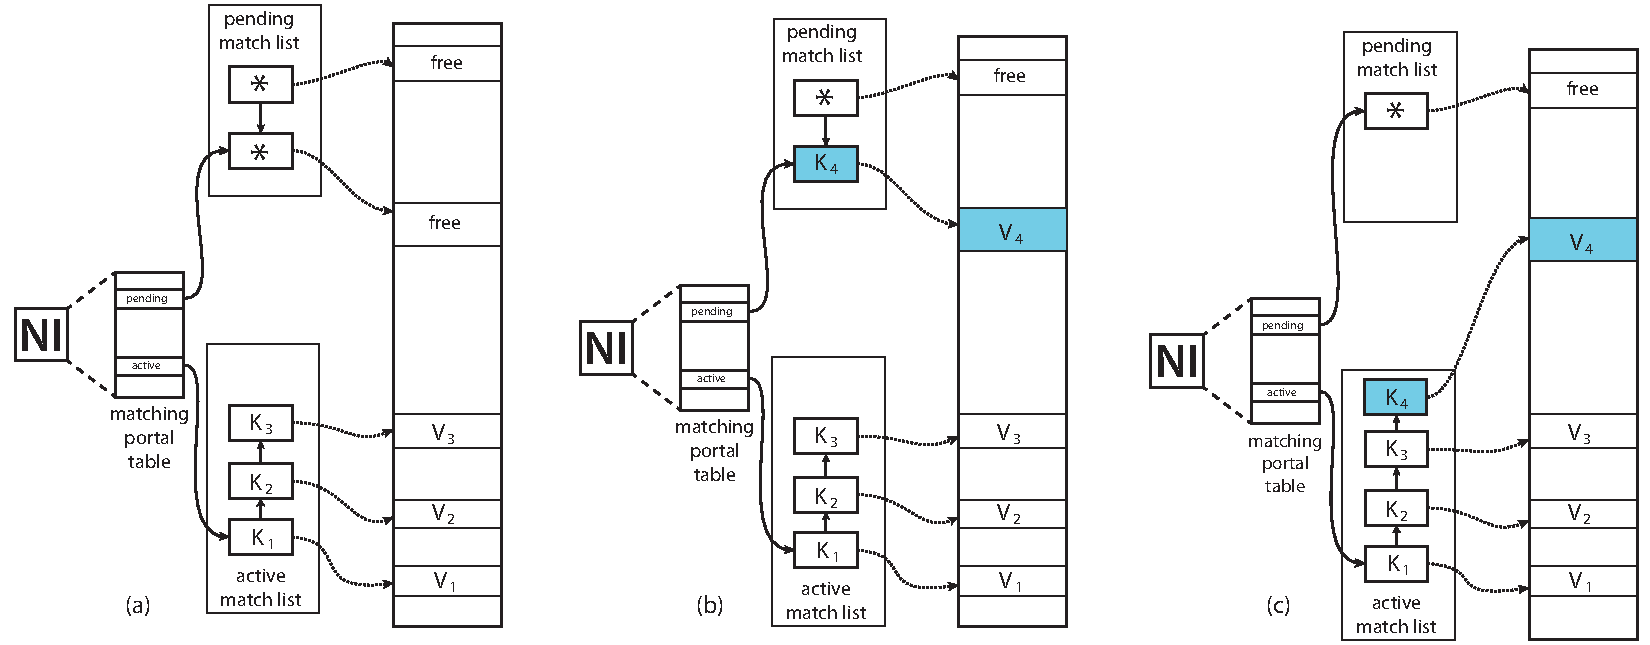
\includegraphics[width=0.85\linewidth]{figs/put}
  \caption{Sequence of target-side actions performed during a \pdht~{\tt insert()} operation.}
  \label{fig:put}
\end{figure*}

The progress thread is a viable approach for handling insertion requests, but
requires target-side processing by both Portals and PDHT. Portals provides an
experimental feature that allows for a triggered match list append operation to
occur when an event counter exceeds a specified threshold value. We can
eliminate the progress thread altogether by using these {\em triggered append}
operations. In this approach, PDHT key/value match list and table entries are
associated with a Portals event counter, initially zero.  When the wildcard MEs
are created on the pending list, triggered append operations are also setup to
trigger when the wildcard ME is written to. This allows the Portals layer to be
responsible for moving key/value pairs from the pending list over to the active
list. One issue with this approach is that Portals requires the match bits for
the appended entry to be specified at setup time, rather than when the trigger
is executed. This can be worked around with the current reference
implementation, or by using multiple triggered operations. We are in the
process of proposing additional triggered operations and semantics to the Portals
specification, in order to ensure that these applications can be efficiently
implemented with hardware offload systems.

\subsection{Accessing Objects}

In contrast to the complexity of adding new items to the PDHT, other
operations, such as reading or updating, are straightforward. PDHT supports
get, update, and atomic update operations on key/value pairs.  When an
operation is requested, the key is hashed to yield the rank and match bits. The
system then simply invokes the corresponding Portals get, put, or atomic
operation on the active match list with the hashed match bits value. Portals
performs the operation and updates an event counter that increments a success
or failure counter. In the case of a failure, PDHT discriminates a "not found"
error from other networking troubles.

\subsection{Match list Performance}

PDHT is able to provide efficient get operations by adding a match list entry
to the Portal table entry. A subsequent get operation causes the target side
to search the match list for a matching entry and returns the data object
associated with the requested match bits field. A significant challenge to 
implementing a large-scale key/value store on top of this approach is that
the match list is conventionally implemented as a linked-list, which much be
searched upon any message request. If a process is hosting a large number
of key/value entries, searching this list may be prohibitively expensive.
Traditional uses of the matching interface, such as implementing MPI message
matching would rarely see match list lengths on the scale as may be used in 
PDHT (one per element) \cite{flajslik:16}.

Indeed, initial results showed that matchlist length had a critical 
impact on the access times within PDHT~\cite{comhpc16}. Our first
approach to deal with this issue was to adapt the hash function
to map a logical key to a tuple including the rank, match bits, and 
a new PTE index value. The PDHT implementation now distributes
key/value objects over multiple Portal table entries. Instead of 
a single entry with a match list containing 10,000 entries, the
system could be configured with 10 PTE match lists, each containing
approximately 1,000 entries. While this simplistic technique did
reduce matchlist overhead, search latency was still noticable, 
especially on small scale runs, or with very large datasets.


When used in message-passing libraries, the matching procedure must preserve
the ordering of posted communication operations. However, with the PGLAS
approach, no ordering constraint exists and sequentially searching a linked
list unnecessarily slows performance.

The Portals 4 reference implementation as recently accepted a patch
to support unordered matching operations on a Portals matching interface.
This was implemented by adding a new option that is specified when
creating a new PTE. When this option is activated, the matchlist
append operation stores a refrence to the ME in a lightweight 
hash table~\cite{uthash}.  The search process is also amended to circumvent 
a list traversal by first checking the hash table for a matching entry.
This results in much improved performance with respect to the initial
implementation.

\subsection{Hash Collisions} 

A hash collision occurs when multiple keys map to an identical rank/match bits
pair. By default, PDHT detects collisions by comparing the requested key value
against the key of the retrieved object and reporting the condition to the
application. PDHT can handle collisions transparently within the system, but
this is not a problem in practice.

In traditional hash tables, a hashed key, $K$, is used with modular arithmetic
to select a location in an array of elements of size $N$. The hash function
provides a mapping between $K \rightarrow N$ elements.  If the size of the key
space, $|K|$, is much larger than $N$, the likelihood of collisions increases.
Conventional approaches are to store a list of objects within each array entry
(chaining) to limit the overhead of collisions.

While PDHT also uses an array to hold the collection of hash table entries, the
indexing into this array is performed indirectly, by Portals. At
initialization, match list entries are created that map to specific table
entries. While each table may be of size $N$, each of the $N$ entries is
indexed by the Portals match bits value, using a hash function that maps from
$K \rightarrow 2^{64}$. Compared to traditional implementations, $N \ll
2^{64}$, which has the impact of dramatically lowering the probability of a
collision, given a reasonable hash function.


% get operation
%  - run hash
%  - issue PtlGet from active list
%  - check for collision



%  - custom hash functions 
%  - 64-bit hash space, rather than array bucket
%      - detach key -> array size dependency
%      - lower collision rates

% other operations
%  - iteration
%  - non-blocking / bundled puts/gets
%  - interoperability


%%% Local Variables: 
%%% mode: latex
%%% TeX-master: "paper"
%%% End: 
